\fancypagestyle{plain}{\fancyhead{}\renewcommand{\headrulewidth}{0pt}}
\chapter{Esperimenti}
Ultimata l’implementazione del codice, ora più facilmente fruibile grazie alla creazione del file \texttt{.lib}, il passo successivo riguarda lo sviluppo di applicazioni vere e proprie in grado di fare affidamento sulla libreria Edge Engine. In particolare, questo capitolo prende in considerazione tre esperimenti differenti: il primo tratta un esempio di utilizzo su PC Windows (più completo e significativo rispetto a quello descritto nella sezione \ref{prova}), il secondo verte invece sulla creazione di un plugin che permetta di usufruire della libreria anche in ambiente Unity3D e, infine, il terzo descrive un vero e proprio caso applicativo portato a termine da due tesisti triennali del corso di Ingegneria Elettronica e Tecnologie dell'Informazione dell'Università degli Studi di Genova.
\section{Applicazione Windows}
L'esempio di utilizzo per Windows è stato creato al fine di mostrare e testare tutte le potenzialità offerte dall'allargamento del pool di piattaforme supportate da Edge Engine.

Come accennato brevemente nella sezione \ref{prova}, in primo luogo è necessario riportare sul Cloud la descrizione della risorsa che si intende adottare. Più in particolare, sono da specificare i parametri mostrati nella tabella seguente:

\begin{table}[H]
	\begin{tabular}{|p{0.15\textwidth}|p{0.44\textwidth}|p{0.32\textwidth}|}
		\hline
		\textbf{Parametri} & \textbf{Nome} & \textbf{URL}\\
		\hline
		\textbf{Thing} & my-pc & {{url}}/v1/things/my-pc\\
		\hline
		\textbf{Feature} & total-ram, total-rom, available-ram, available-rom & {{url}}/v1/features\\
		\hline
		\textbf{Device} & pc-probe & {{url}}/v1/devices/pc-probe\\	
		\hline
		\textbf{Script} & total-rom-installed, total-ram-installed, ram-available, rom-available, average-hourly-available-ram, ram-available-to-mb, rom-available-to-mb,  max-available-ram, max-available-rom & {{url}}/v1/scripts\\	
		\hline
	\end{tabular}
\\\\url = \url{http://students.atmosphere.tools/}
	\caption{Parametri Measurify della risorsa Windows}
	\label{paramMeas}
\end{table}

Il device \texttt{pc-probe} contiene all'interno della sua descrizione le feature e gli script ad esso associati. Le prime indicano grandezze fisiche misurabili dal dispositivo, mentre i secondi rappresentano le funzioni di elaborazione che è possibile applicare ai dati ricevuti. 

La tabella \ref{script} mostra la struttura degli script implementati. Essi sono composti da due campi principali: \texttt{\_id} e \texttt{code}.  \texttt{\_id} specifica il nome associato allo script stesso, mentre \texttt{code} contiene le effettive operazioni che il dispositivo fisico andrà ad effettuare. 

\begin{table}[H]
	\begin{tabular}{|p{0.27\textwidth}|p{0.67\textwidth}|}
		\hline
		\textbf{\_id} & \textbf{code} \\
		\hline
		ram-available & available-ram().send()\\
		\hline
		rom-available & available-rom().send()\\
		\hline
		total-ram-installed & total-ram().send()\\
		\hline
		total-rom-installed & total-rom().send()\\
		\hline
		max-available-ram & available-ram(10).max().send()\\	
		\hline
		max-available-rom & available-rom(10).max().send()\\
		\hline	
		ram-available-to-mb & available-ram().map(a*1024).send()\\
		\hline
		rom-available-to-mb & available-rom().map(a*1024).send()\\
		\hline
		average-hourly-available-ram & available-ram(6m).window(+,0,10).map(a/10).send()\\
		\hline
	\end{tabular}
	\caption{Script correlati al device \texttt{pc-probe}}
	\label{script}
\end{table}

Prendendo ad esempio lo script \texttt{ram-available-to-mb}, il codice in oggetto permette di ricavare la quantità, espressa in gigabyte, di memoria RAM disponibile tramite l’operazione \texttt{available-ram()}, la quale viene poi concatenata a \texttt{map(a*1024)}, che converte il valore ottenuto in megabyte, moltiplicandolo per un fattore 1024. Infine, tramite la \texttt{send()}, il campione appena elaborato viene inviato a Measurify.

Lo script \texttt{average-hourly-available-ram}, invece, calcola la media oraria di RAM disponibile, ma necessita di un tempo di elaborazione più lungo di una singola esecuzione dell'engine, come specificato dal codice:\\ \texttt{available-ram(6m).window(+,0,10).map(a/10).send()}\\ L’operazione \texttt{available-ram(6m)} permette di campionare ogni sei minuti. Tramite la \texttt{window(+,0,10)} poi, viene presa una finestra di dieci input e calcolata la somma di tali elementi. Il calcolo della media viene poi portato a termine grazie alla \texttt{map(a/10)}, che opera una divisione sul totale per il numero di campioni presi in considerazione. Infine, il risultato viene inviato al Cloud grazie alla \texttt{send()}.

Una volta riportata su Measurify la descrizione della risorsa di cui si intende usufruire, è possibile passare allo sviluppo del codice dell'applicazione. Si hanno nuovamente due funzioni principali, \texttt{setup} e \texttt{action}, che svolgono gli stessi task di autenticazione, elaborazione e invio dei dati descritti nella sezione \ref{prova}. In questo caso però, \texttt{action} viene eseguita ciclicamente per un numero di volte specificato dalla variabile \texttt{loopCount}. Ciò al fine di poter disporre di un tempo di esecuzione più lungo, nel caso in cui si desideri, ad esempio, usufruire dello script \texttt{average-hourly-available-ram}, il quale richiede un'ora di tempo per la collezione dei campioni.

Inoltre, al fine di recuperare dalla macchina in uso le informazioni relative all'utilizzo delle memorie RAM e ROM, sono state implementate le funzioni \texttt{getRAMinfo} e  \texttt{getROMinfo}. Esse sono esclusive per piattaforme dotate di sistema operativo Windows, in quanto fanno uso della libreria proprietaria. Qualora si riveli necessario modificare il progetto volendolo adattare ad altri OS, sarà sufficiente sostituire le suddette funzioni con altre, specifiche del target desiderato.

Un esempio di dato conservato sul Cloud, elaborato dallo script \\\texttt{ram-available-to-mb} del device \texttt{my-pc} è mostrato in figura \ref{datowin}.

\begin{figure}[H]
	\centering
	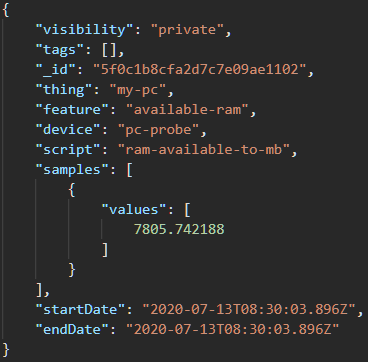
\includegraphics[scale=0.7]{pics/datowin}
	\caption{Dato relativo al valore di memoria RAM disponibile convertito in MB e conservato sul Cloud}
	\label{datowin}
\end{figure}

\section{Applicazione alla Realtà Virtuale}
Edge Engine nasce dall'idea di voler offrire uno strumento modulare e slegato dall'hardware che possa facilitare e incentivare lo sviluppo di applicazioni IoT. Questo motore, oltre ad essere una valida soluzione per tale scopo, potrebbe inoltre risultare ugualmente efficace in un contesto totalmente differente, come quello dei videogiochi. Ciò è dovuto al fatto che, attualmente, non esiste uno strumento che elabori al tempo stesso dati provenienti da sorgenti così eterogenee come possono apparire un sensore fisico ed uno presente all'interno di un mondo virtuale. Si pensi per esempio ad un videogiocatore che abbia intenzione di monitorare il proprio battito cardiaco e, al contempo, processare dati provenienti dall'ambiente di gioco. Edge Engine, se adattato ad un Integrated Development Environment (IDE) dedito alla creazione di videogiochi, potrebbe essere in grado di svolgere entrambi i task richiesti, grazie all'alto livello di scalabilità di cui dispone.

Come ulteriore obbiettivo, dunque, si intende trattare lo sviluppo di un'applicazione per Unity3D con lo scopo di poter così osservare il funzionamento di Edge Engine in un contesto, la realtà virtuale, diverso da quello per cui è stato inizialmente pensato, ma che può spesso rivelarsi strettamente collegato, o collegabile, all'ambiente reale.

In primo luogo verranno descritti i passi richiesti per la creazione di un plugin, necessario al fine di utilizzare Edge Engine all'interno dell'ambiente Unity3D. In seconda istanza poi, sarà discussa l'implementazione di un'applicazione esemplificativa che sfrutti il plugin in precedenza sviluppato.
\subsection{Plugin}\label{plugin}
All'interno di Unity, normalmente si utilizzano gli script C\# per la creazione di funzionalità, ma è anche possibile includere codice creato al di fuori di Unity sotto forma di plugin. I plugin sono librerie di codice nativo specifiche della piattaforma. Possono accedere a funzionalità quali chiamate del sistema operativo e librerie di codici di terze parti che altrimenti non sarebbero disponibili per Unity. Tuttavia, queste librerie non sono accessibili agli strumenti di Unity come le normali librerie utilizzabili all'interno dell'IDE.

Per la creazione del plugin di Edge Engine, che corrisponde in tutto e per tutto ad una Dynamic-Link Library (DLL), si è scelto di utilizzare Visual Studio, data l'affinità di tale IDE con Unity. Dal momento che il compilatore offerto da Visual Studio, MSVC, è differente da g++ (usato in precedenza per la creazione della libreria Edge Engine e l’installazione delle librerie POCO), è stato in primo luogo necessario ricompilare entrambi i progetti.

Per quanto riguarda le librerie POCO, in questo caso, siccome il compilatore proposto di default da VCPKG è proprio MSVC, in quanto sviluppati entrambi da Microsoft, si è deciso di utilizzare questo package manager, scegliendo la versione a 64 bit. Rispetto ai problemi riscontrati in precedenza con il compilatore g++, l’installazione delle librerie è andata a buon fine senza alcun intoppo. Per la compilazione è necessario eseguire i seguenti comandi:

\begin{verbatim}
vcpkg install poco:x64-windows
vcpkg integrate install
\end{verbatim}

Il comando di \texttt{integrate install} non è obbligatorio, ma semplifica l'utilizzo delle librerie POCO all'interno dei progetti, evitando allo sviluppatore di dover inserire le locazioni degli header e dei file \texttt{.lib}, necessari alla compilazione.

Per quanto riguarda invece la libreria Edge Engine, è stato creato nuovamente un file \texttt{.lib}, ma questa volta, facendo affidamento a MSVC per i motivi sopracitati. Per poter poi utilizzare tale libreria all'interno del progetto di creazione della DLL, è stato necessario fornire al compilatore, tramite la schermata di impostazioni di Visual Studio, la locazione degli header e del file \texttt{Edgine.lib}.

Una volta poste le basi per la creazione della libreria dinamica che sarebbe poi stat utilizzata come plugin all'interno di Unity, è stato possibile passare alla fase di implementazione della stessa.

Lo schema della DLL che è stata prodotta prevede una singola classe, dentro la quale sono presenti le funzioni a cui si intende poi fare riferimento dal lato C\# e il relativo header. All'interno di quest'ultimo, è necessario definire tali funzioni con l’attributo \texttt{\_\_declspec(dllexport)}, il quale indica che esse possono essere chiamate dallo script che sfrutta il plugin. Inoltre, tramite la keyword \texttt{extern "C"}, si indica al compilatore che le funzioni in oggetto devono impiegare la convenzione di linking del linguaggio C. Ciò è necessario al fine di esportarle correttamente, altrimenti, a causa del mangling operato dai compilatori C++, non sarebbe poi possibile far riferimento ad esse in ambiente Unity. Il mangling è una tecnica utilizzata per distinguere funzioni che hanno lo stesso nome (overloading). Essa consiste nella manipolazione del nome in fase di compilazione affinché esso sia univoco, ma, in questo specifico caso, ciò renderebbe ignoto allo sviluppatore il nome definitivo associato e, per questo motivo, non sarebbe poi in grado di utilizzare tali funzioni all'interno del plugin. Il linguaggio C, invece, non prevede il mangling delle funzioni, dal momento che la tecnica di overload non è supportata. Pertanto, il file binario generato dalla compilazione contiene i nomi originali delle funzioni esportate, che possono essere chiamate dal lato C\# senza incongruenze. Siccome la convenzione di linking adottata è quella del linguaggio C, è necessario che, nonostante il corpo delle funzioni sia scritto in C++, i tipi di dato di input e output siano quelli propri del C.

Andando, come di consueto, a riprendere la struttura degli sketch Arduino, si è scelto di implementare due funzioni esportabili: \texttt{Setup} e \texttt{Action}. Il loro funzionamento è analogo ai casi precedentemente discussi, con un’importante differenza relativa all'inserimento delle caratteristiche descrittive, quali \textit{device}, \textit{thing}, \textit{feature}, \textit{username} e \textit{password}. In questo specifico caso infatti, se prima tali informazioni era necessario inserirle all'interno del codice, ora si è scelto di renderle configurabili da parte dell'utente dal lato Unity. Di seguito sono mostrate le firme delle due funzioni in oggetto:

\begin{verbatim}
void Setup(char* myId, char* myPw, char* myThing, char* myDevice,
           char* myDeviceId)
void Action(char* sampleName, float hits)
\end{verbatim}

La \texttt{Setup} prende in ingresso nell'ordine \textit{username}, \textit{password}, \textit{thing}, \textit{device}  e \textit{deviceId}, un identificativo univoco per ogni dispositivo.

La \texttt{Action}, invece, riceve il nome della \textit{feature} e il relativo dato misurato per poterlo processare e inviare successivamente al Cloud.

Il progetto così compilato produce i file \texttt{NATIVECPPLIBRARY.dll}, \\\texttt{pcred.dll}, \texttt{PocoFoundationd.dll}, \texttt{PocoNetd.dll}, \texttt{zlibd1.dll}. Il primo rappresenta proprio la libreria dinamica contenente le funzioni appena create che vengono poi utilizzate all'interno di uno script Unity. Il secondo, invece, è una DLL di file si sistema essenziali dell'OS Windows. Infine, gli ultimi tre sono un’elaborazione, operata durante la creazione della DLL, delle librerie POCO, necessarie al funzionamento di  \texttt{NATIVECPPLIBRARY.dll}. Al fine di utilizzare all'interno di Unity la DLL appena creata, è necessario copiare questi file dentro la cartella di progetto.
\subsection{Unity}

\begin{figure}[H]
	\centering
	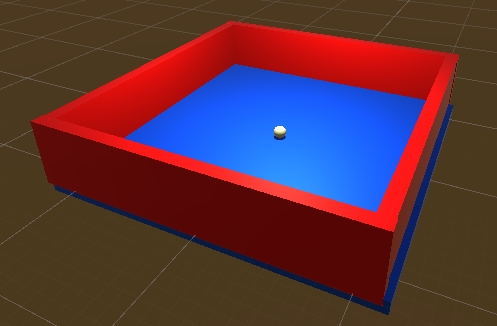
\includegraphics[scale=1.1]{pics/ring}
	\caption{Scena di gioco Unity3D}
	\label{ring}
\end{figure}

Sul fronte Unity, avendo come obbiettivo primario il test delle funzionalità di Edge Engine anche in un contesto di realtà virtuale, si è deciso di creare una semplice applicazione di esempio in grado di raccogliere dati provenienti dalla scena di gioco e, tramite il plugin descritto precedentemente, di inviarli a Measurify. In particolare, è stato creato un ring contenente al suo interno una pallina controllabile tramite i tasti freccia del PC (si veda fig. \ref{ring}). Ogniqualvolta la pallina urta uno dei quattro muri delimitanti, la collisione viene registrata all'interno di una variabile incrementale e, in caso di raggiungimento di un numero di collisioni multiplo di cinque (lo zero è escluso per ovvi motivi), tale valore viene inviato al Cloud. Come si può facilmente dedurre, tale applicazione, differentemente da quella per Windows, rappresenta un mero esempio di utilizzo di Edge Engine all'interno dell'ambiente di gioco e non intende in alcun modo mostrare un vero e proprio caso applicativo, dal momento che non è questo lo scopo del progetto Unity.

In primo luogo, è stato necessario inserire la descrizione della risorsa all'interno di Measurify, riassunta in tabella \ref{descunitydev}.

\begin{table}[H]
	\begin{tabular}{|p{0.15\textwidth}|p{0.30\textwidth}|p{0.46\textwidth}|}
		\hline
		\textbf{Parametri} & \textbf{Nome} & \textbf{URL}\\
		\hline
		\textbf{Thing} & ball & {{url}}/v1/things/ball\\
		\hline
		\textbf{Feature} & collision & {{url}}/v1/features/collision\\
		\hline
		\textbf{Device} & unityDevice & {{url}}/v1/devices/unityDevice\\    
		\hline
		\textbf{Script} & collisions-count-send & {{url}}/v1/scripts/collisions-count-send\\    
		\hline
	\end{tabular}
	\\\\url = \url{http://students.atmosphere.tools/}
	\caption{Parametri Measurify della risorsa Unity}
	\label{descunitydev}
\end{table}

Come spiegato in precedenza, siccome quest'applicazione è pensata per essere un semplice esempio guida, il valore associato alla sola feature \texttt{collision} viene inviato così com'è, senza alcuna elaborazione intermedia.

Veniamo dunque allo sviluppo dello script C\# che permette la fruizione della libreria Edge Engine anche all'interno di Unity.  

\begin{wrapfigure}{r}{7.5cm}
	\centering
	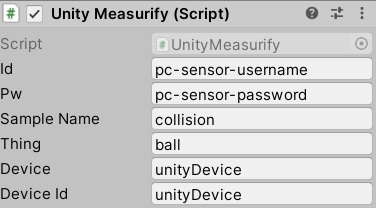
\includegraphics[scale=0.85]{pics/unityscriptvars}
	\caption{\centering{Variabili settabili dall'utente all'interno dell'inspector Unity}}
	\label{unityscriptvars}
\end{wrapfigure}

Ricordando la struttura delle funzioni esportate dal plugin mostrata nella sezione \ref{plugin}, le quali prevedono di ricevere in ingresso i nomi dei parametri descrittivi della risorsa, oltre alle credenziali di accesso, al fine di mantenere un elevato livello di configurabilità, si è scelto di impostare queste variabili come settabili da parte dell'utente dichiarandole \texttt{public}, come visibile in figura \ref{unityscriptvars}. Così facendo, lo sviluppatore è in grado di personalizzare a piacere i dettagli relativi al proprio caso applicativo.

Successivamente, per poter far uso all'interno di Unity delle funzioni \texttt{Setup} e \texttt{Action}, esposte dal plugin, è necessario dichiararle con l’attributo \texttt{DLLImport}, come mostrato di seguito:

\begin{verbatim}
[DllImport("NATIVECPPLIBRARY", EntryPoint = "Setup")]
public static extern void Setup(StringBuilder myId, 
StringBuilder myPw, StringBuilder myThing, 
StringBuilder myDevice, StringBuilder myDeviceId);

[DllImport("NATIVECPPLIBRARY", EntryPoint = "Action")]
public static extern void Action(StringBuilder mySample, 
float data);
\end{verbatim}

\begin{itemize}
	\item \texttt{DLLImport} indica l'importazione da una DLL;
	\item \texttt{EntryPoint} fornisce al compilatore il nome che la funzione ha all'interno del plugin;
	\item \texttt{extern} è un attributo necessario per dichiarare una funzione che è implementata esternamente.
\end{itemize}

Come è possibile notare, il passaggio dei parametri testuali avviene per lo più attraverso dati di tipo \texttt{StringBuilder}. Ciò è dovuto al fatto che l’utilizzo della memoria di \texttt{StringBuilder} e array di \texttt{char} è simile, pertanto il plugin è in grado di interpretare correttamente il contenuto del primo definito dal lato Unity. 

Come di consueto, lo script Unity è organizzato nel seguente modo: un metodo \texttt{Start}, che viene eseguito una sola volta all’avvio del programma, e uno, \texttt{Update}, che viene invece ripetuto ciclicamente. Dal momento che, anche in questo caso, lo schema di base è simile a quello degli sketch Arduino, va da sé che la funzione \texttt{Setup} verrà chiamata all'interno di \texttt{Start}, mentre la \texttt{Action} dentro \texttt{Update}, come visibile in figura \ref{startupdate}. 

\begin{figure}[H]
	\centering
	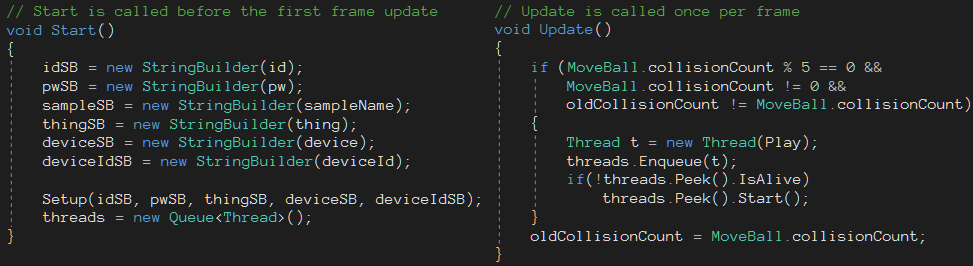
\includegraphics[width=\linewidth]{pics/startupdate}
	\caption{Metodi \texttt{Start} e \texttt{Update} dello script Unity}
	\label{startupdate}
\end{figure}

\texttt{Start} ha il compito di inizializzare tutte le variabili pubbliche di tipo \texttt{StringBuilder} coinvolte nello script. Una volta recuperati i parametri inseriti dall'utente, viene eseguita la \texttt{Setup} che, si rammenta, permette di autenticarsi su Measurify ottenendo il JWT per gli accessi successivi. In ultimo, viene inizializzato un oggetto di tipo \texttt{Queue<Thread>} che si occupa di gestire le future chiamate della funzione \texttt{Action}. La creazione di oggetti di tipo \texttt{Thread} è necessaria in quanto, altrimenti, la normale esecuzione del programma verrebbe interrotta per qualche istante ad ogni invio dei dati al Cloud, a causa del tempo necessario a compiere questo task. Grazie all'utilizzo dei thread, l'applicazione può continuare il suo normale svolgimento mentre, in parallelo, la funzione \texttt{Action} viene portata a termine. I thread vengono inseriti all'interno di una coda al fine di ottenere una più semplice gestione degli stessi, avendo la possibilità di crearli, eseguirli e distruggerli in modo ordinato facendo uso dei metodi \texttt{Enqueue}, \texttt{Peek} e \texttt{Dequeue}.

\texttt{Update}, innanzitutto, esegue un controllo relativo al numero di collisioni che la pallina ha effettuato. Tale valore deve essere multiplo di cinque, diverso da zero e differente dal dato precedentemente inviato al Cloud, in modo da non avere duplicati. Se queste tre condizioni sono soddisfatte, viene creato un nuovo thread e aggiunto alla coda. A meno che il programma non ne stia già eseguendo uno precedentemente creato, il thread viene eseguito. Tutti quelli rimasti nella coda alla chiusura dell'applicazione vengono lanciati, prima dell'effettivo termine del programma, dal metodo \texttt{OnApplicationQuit}. In questo modo l'applicazione, a regime, non è sovraccarica di un eccessivo numero di thread e, al contempo, viene garantita l'esecuzione di ciascuno di essi entro la conclusione del programma, momento in cui l'utente non interagisce più con la scena di gioco.

Dall'immagine mostrata in figura \ref{risorsaunity} si può notare come, grazie alla creazione del plugin e all'implementazione di uno script che sfrutta tale DLL, Edge Engine sia ora in grado di comunicare correttamente con Measurify anche quando utilizzato in un contesto di realtà virtuale.

\begin{figure}[H]
	\centering
	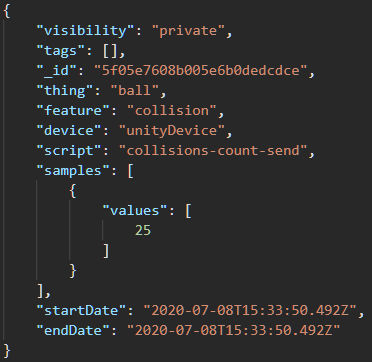
\includegraphics[scale=0.7]{pics/measunity}
	\caption{Dato relativo al numero di collisioni effettuate dalla pallina conservato sul Cloud}
	\label{risorsaunity}
\end{figure}

\subsection{Applicazione reale}
Questa sezione, diversamente da quelle precedenti, non riguarda l’implementazione di Edge Engine su nuove piattaforme, bensì l’utilizzo di tale sistema da parte di due tesisti triennali. In particolare, il progetto in questione tratta di un rilevatore di movimento, composto da un sensore PIR HC-SR501 installato su scheda Arduino ESP8266, il quale necessita di comunicare con il Cloud Measurify per potervi inviare i dati registrati dall'ambiente circostante (si veda fig. \ref{esp8266cloud}). Le potenzialità offerte da Edge Engine risultano adatte allo sviluppo di un’applicazione del genere, siccome la gestione delle HTTP requests viene interamente gestita dall'engine, permettendo dunque agli sviluppatori di adoperarsi maggiormente sugli aspetti di collegamento sensore - board.

\begin{figure}[H]
	\centering
	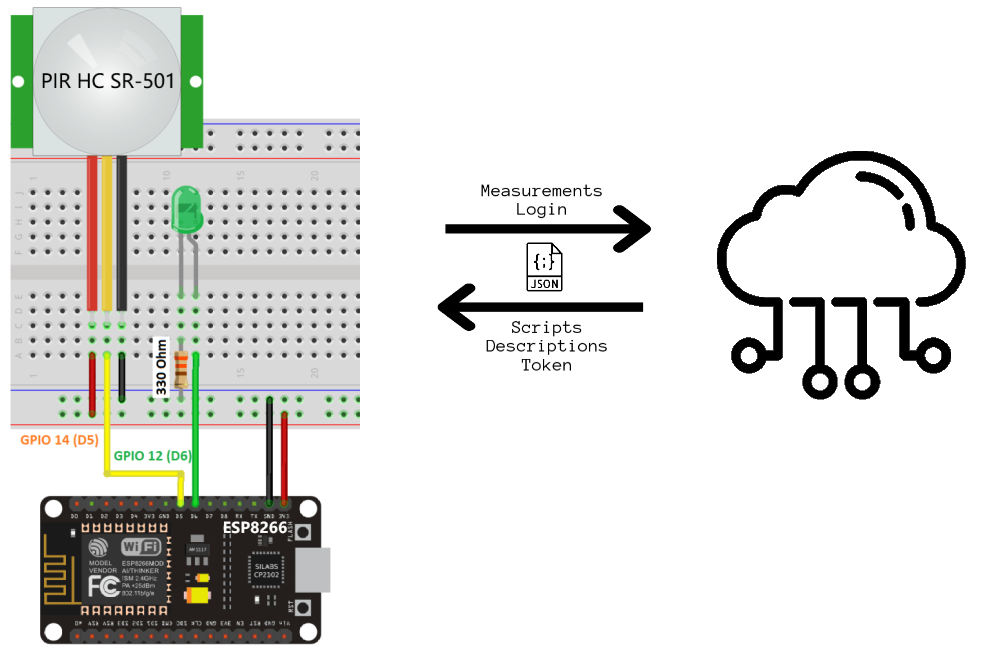
\includegraphics[width=\linewidth]{pics/esp8266cloud}
	\caption{Schema funzionale di Edge Engine per Arduino}
	\label{esp8266cloud}
\end{figure}

Riguardo proprio la comunicazione tra sensore e board, che avviene tramite Interrupt Service Routine (ISR), si è resa peraltro necessaria una piccola modifica al codice sorgente di Edge Engine. In particolare, nella funzione \texttt{getActualDate} della classe \texttt{APIRest}, chiamata proprio all'interno della ISR, veniva definita una variabile di tipo \texttt{float}. Tuttavia, l'utilizzo di tale tipologia di dato all'interno degli interrupt causa la seguente eccezione del coprocessore:

\begin{verbatim}
Guru Meditation Error: 
Core 1 panic'ed (Coprocessor exception [...])
\end{verbatim}

Ciò è dovuto all'intervento della Floating-Point Unit (FPU), non supportata all'interno della ISR. Pertanto, la soluzione adottata è stata la sostituzione del tipo \texttt{float} con \texttt{long} che, non essendo a virgola mobile, non presenta questa problematica.

Una volta risolto questo bug nel codice, è possibile comunicare correttamente con Measurify, come testimoniato dalla figura \ref{measacquario}.

\begin{figure}[H]
	\centering
	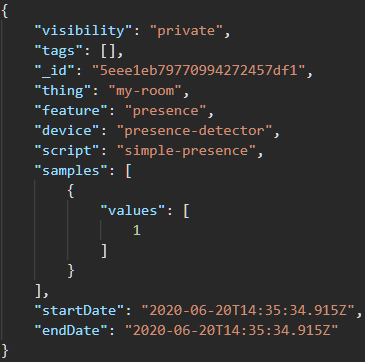
\includegraphics[width=0.6\linewidth]{pics/measacquario}
	\caption{Dato relativo al rilevamento di presenza effettuato dal sensore PIR}
	\label{measacquario}
\end{figure}

Come previsto, i benefici riscontrati dall'utilizzo di Edge Engine, a detta dei diretti interessati, sono stati molteplici. In primo luogo, la facilità d'uso e installazione del sistema ha permesso di concentrarsi maggiormente sul recupero dei dati piuttosto che sugli aspetti della comunicazione Cloud, migliorando così la qualità finale del progetto, riducendo al contempo tempi e quantità di lavoro richiesti. Inoltre, gli esempi di utilizzo forniti hanno permesso di comprendere facilmente come sfruttare il motore perimetrale, fungendo da solida base per lo sviluppo del progetto in questione. Infine, la presenza di script personalizzabili con operazioni concatenabili, nonostante il numero limitato di questi, ha permesso di raggiungere gli obiettivi prefissati in modo logico e preciso.

I principali problemi riscontrati sono stati, invece, la necessità di inserire le credenziali SSID tramite codice e una certa difficoltà di comprensione dell'interazione con il Cloud. In particolare, poiché le richieste HTTP effettuate da Edge Engine sono nascoste all'interno della libreria, non vi è alcun feedback immediato per l'utente in merito alla memorizzazione dei dati su Measurify.

Da questa esperienza di progetto, nonostante vi siano problemi minori da risolvere e ampi margini di miglioramento, si evince come Edge Engine possa essere in grado di offrire una soluzione innovativa e di facile utilizzo adatta anche agli sviluppatori meno esperti che incontrano i tipici problemi relativi alla creazione di un'applicazione IoT.




